\documentclass[12pt]{report}

\usepackage{graphicx}
\usepackage{pdfpages}
\begin{document}

\title{ADS \\  Assignment \#2}
\author{Group 20 \\ Ryan Hart and David Tyler}
\date{\today}
\maketitle

\section*{Objective}
The objective of this laboratory was to create a counter that can count from zero to seven by either even numbers or odd numbers. The current number should then be displayed on a 7--segment display.
\section*{Components}

\begin{itemize}
    \item 1 T74LS157B1 ( 2:1 Multiplexer )
    \item 1 HD74LS04  ( Hex NOT Gate )
    \item 2 HD74LS00  ( Quad NAND Gate )
    \item 1 SN74LS247N  ( 7--Segment Display Decoder )
    \item 1 Toggle Switch ( simulated Clock Signal )
    \item 1 DIP Switch ( 8 Position ON-OFF Single Pole )
    \item 2 SN74L76AD ( Dual JK Flip--Flop )
    \item 1 Dual 7-�Segment Display
    \item 2 $10k\Omega$ resistors
    \item Prototype Board
    \item 5V Power Supply
\end{itemize}

\section*{Experimental Approach}

First, a state table was created with the correct counting logic (taking into account the even/odd buttons for the next state). JK flipflops were used in the design instead of D flipflops. After that, a karnaugh map for both J and K of each of the three flipflops was generated. The minimized logic was then converted into NAND and NOT gates and built. An inverted SR Latch was constructed out of NAND gates to debounce the toggle switch. The outputs from the flipflops were connected to the decoder which was then connected to the seven segment display.

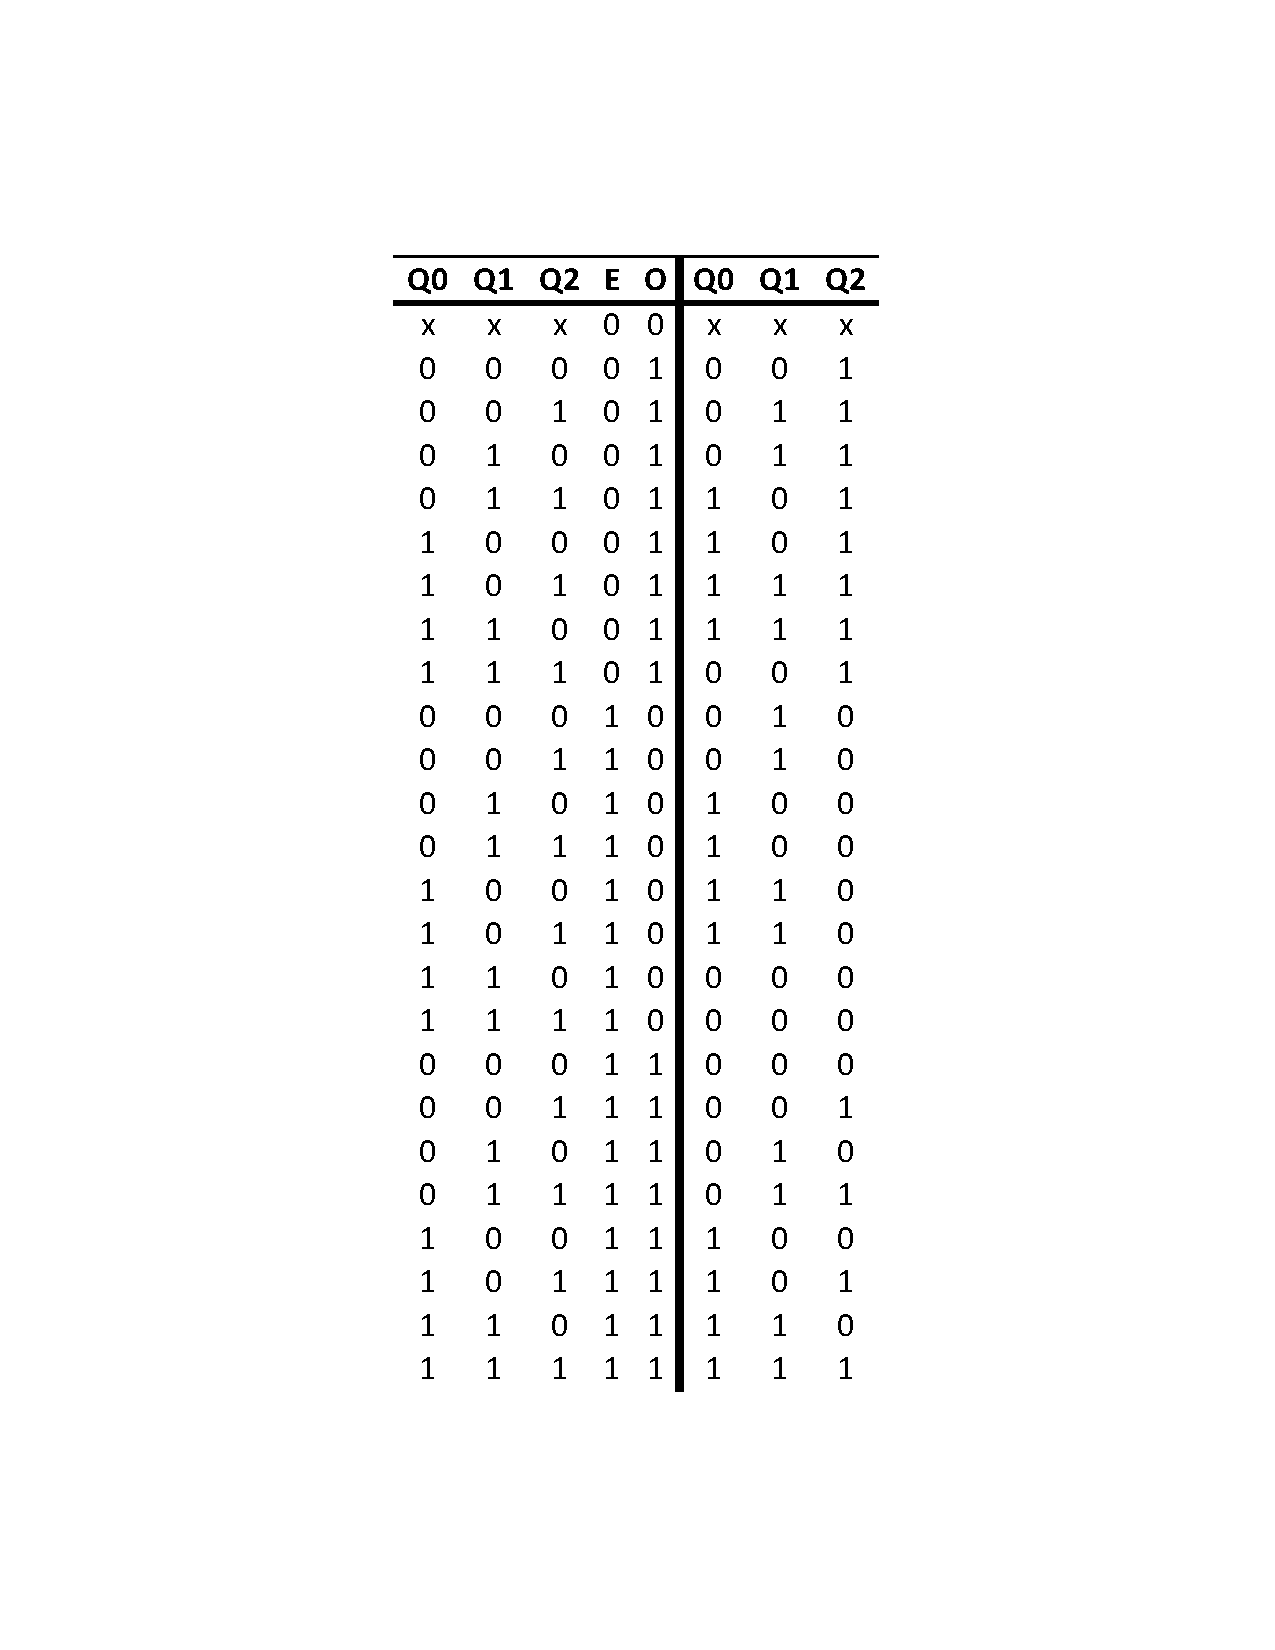
\includepdf[landscape=false, pages=-, scale=0.97]{truthtable.pdf}
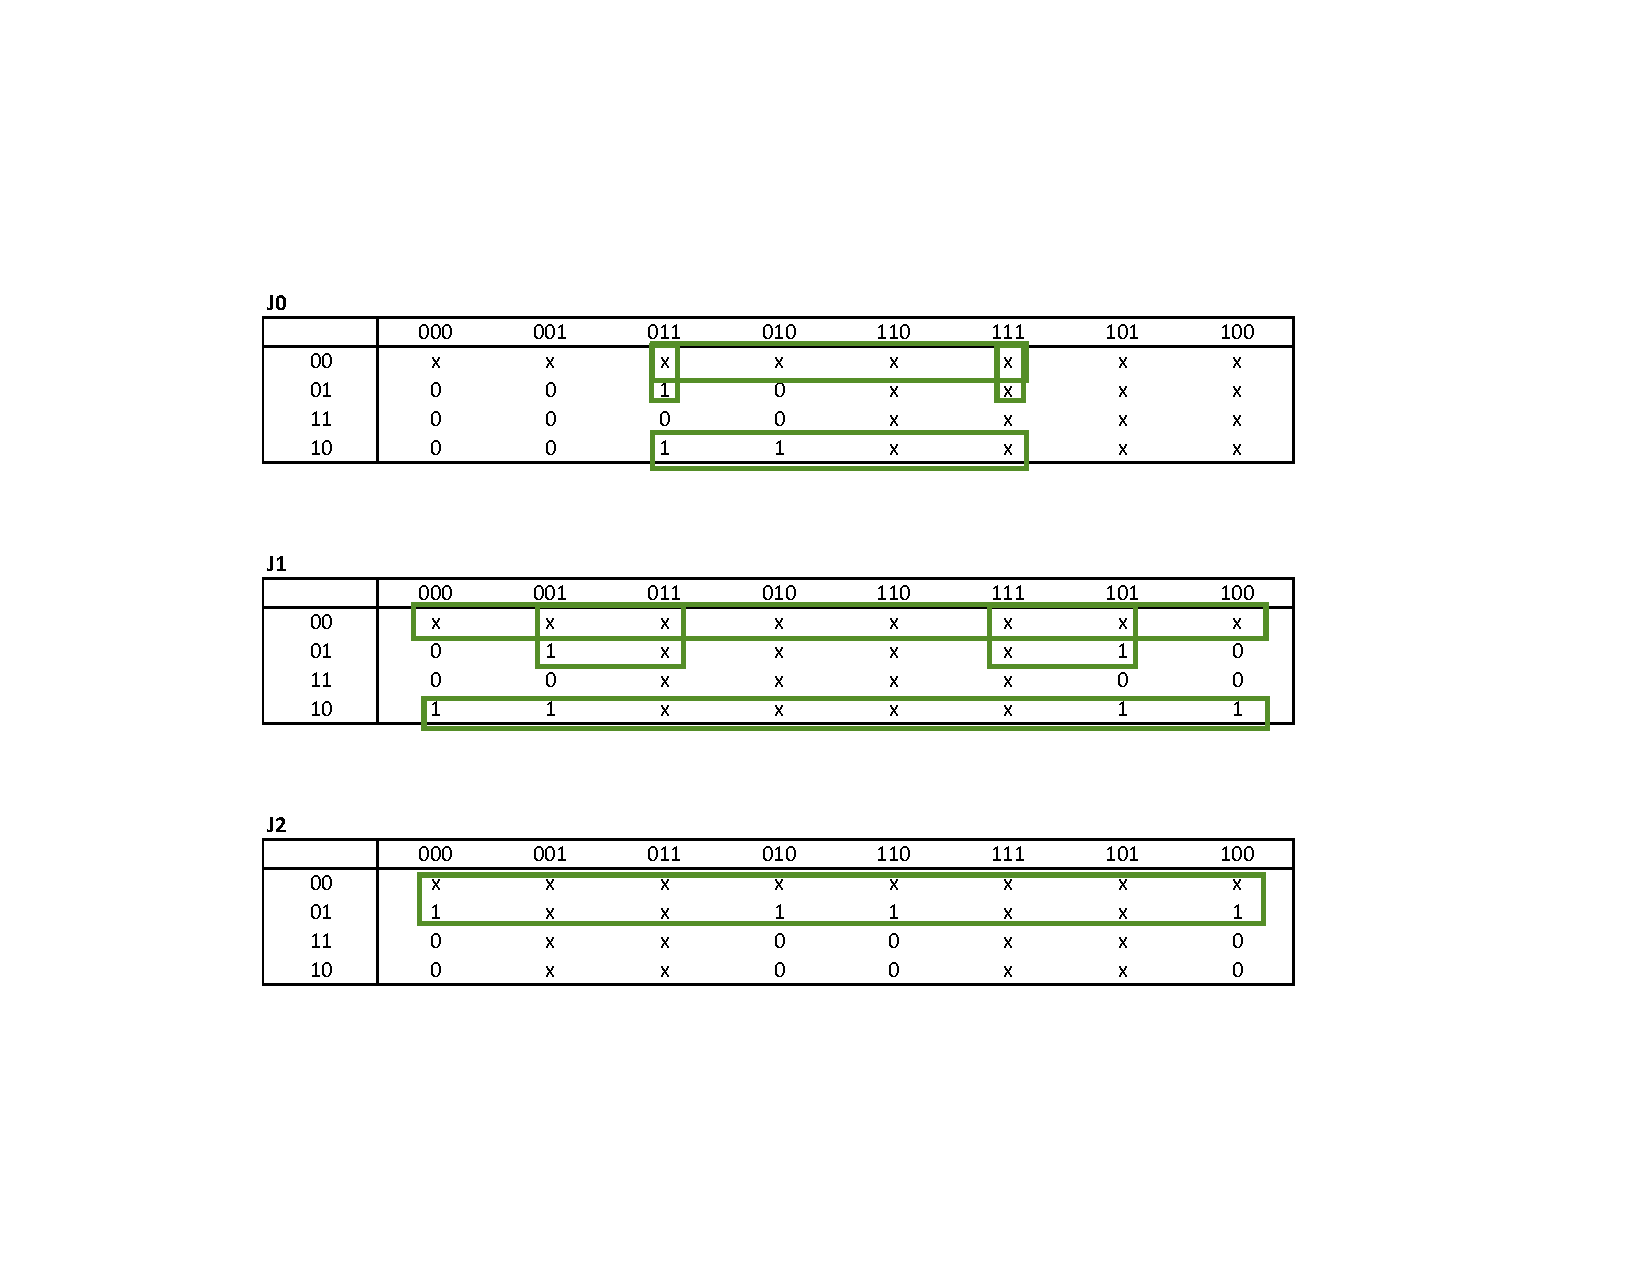
\includepdf[landscape=true, pages=-, scale=0.97]{jmaps.pdf}
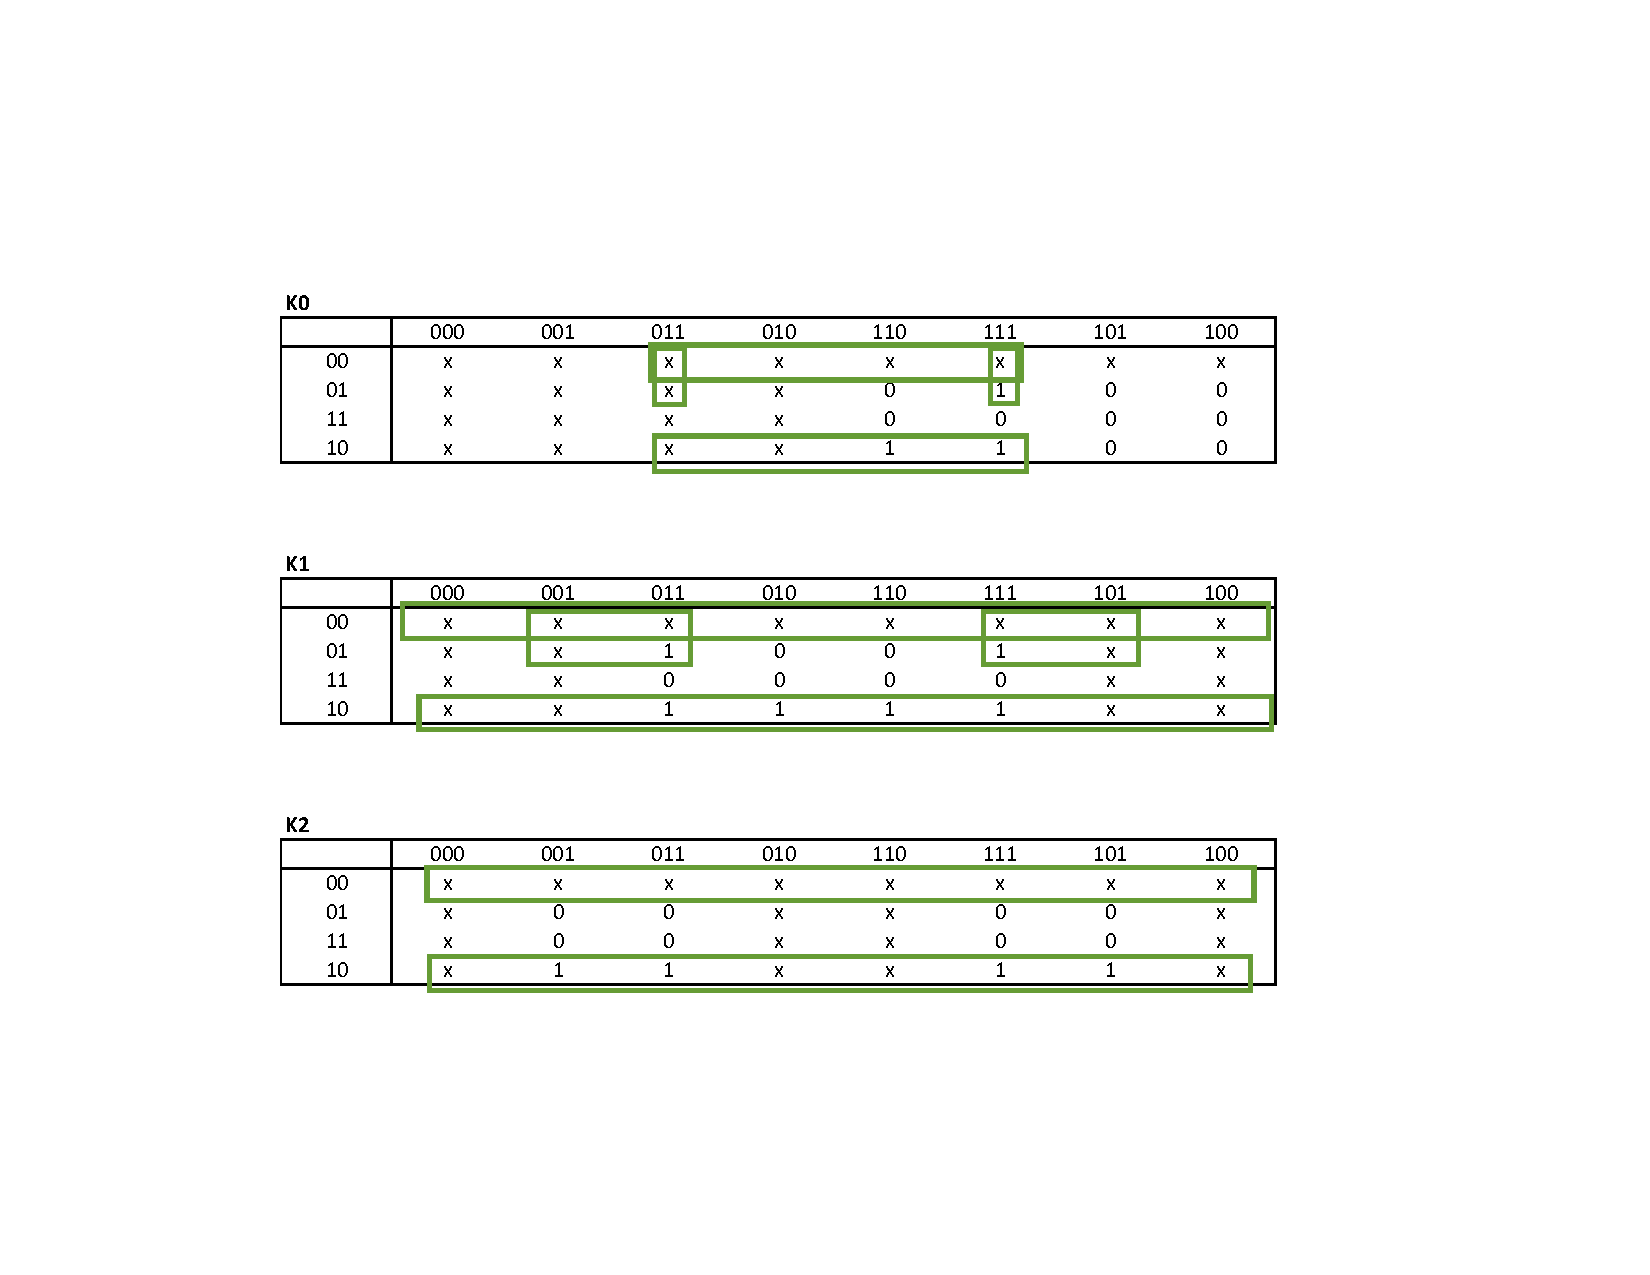
\includepdf[landscape=true, pages=-, scale=0.97]{kmaps.pdf}
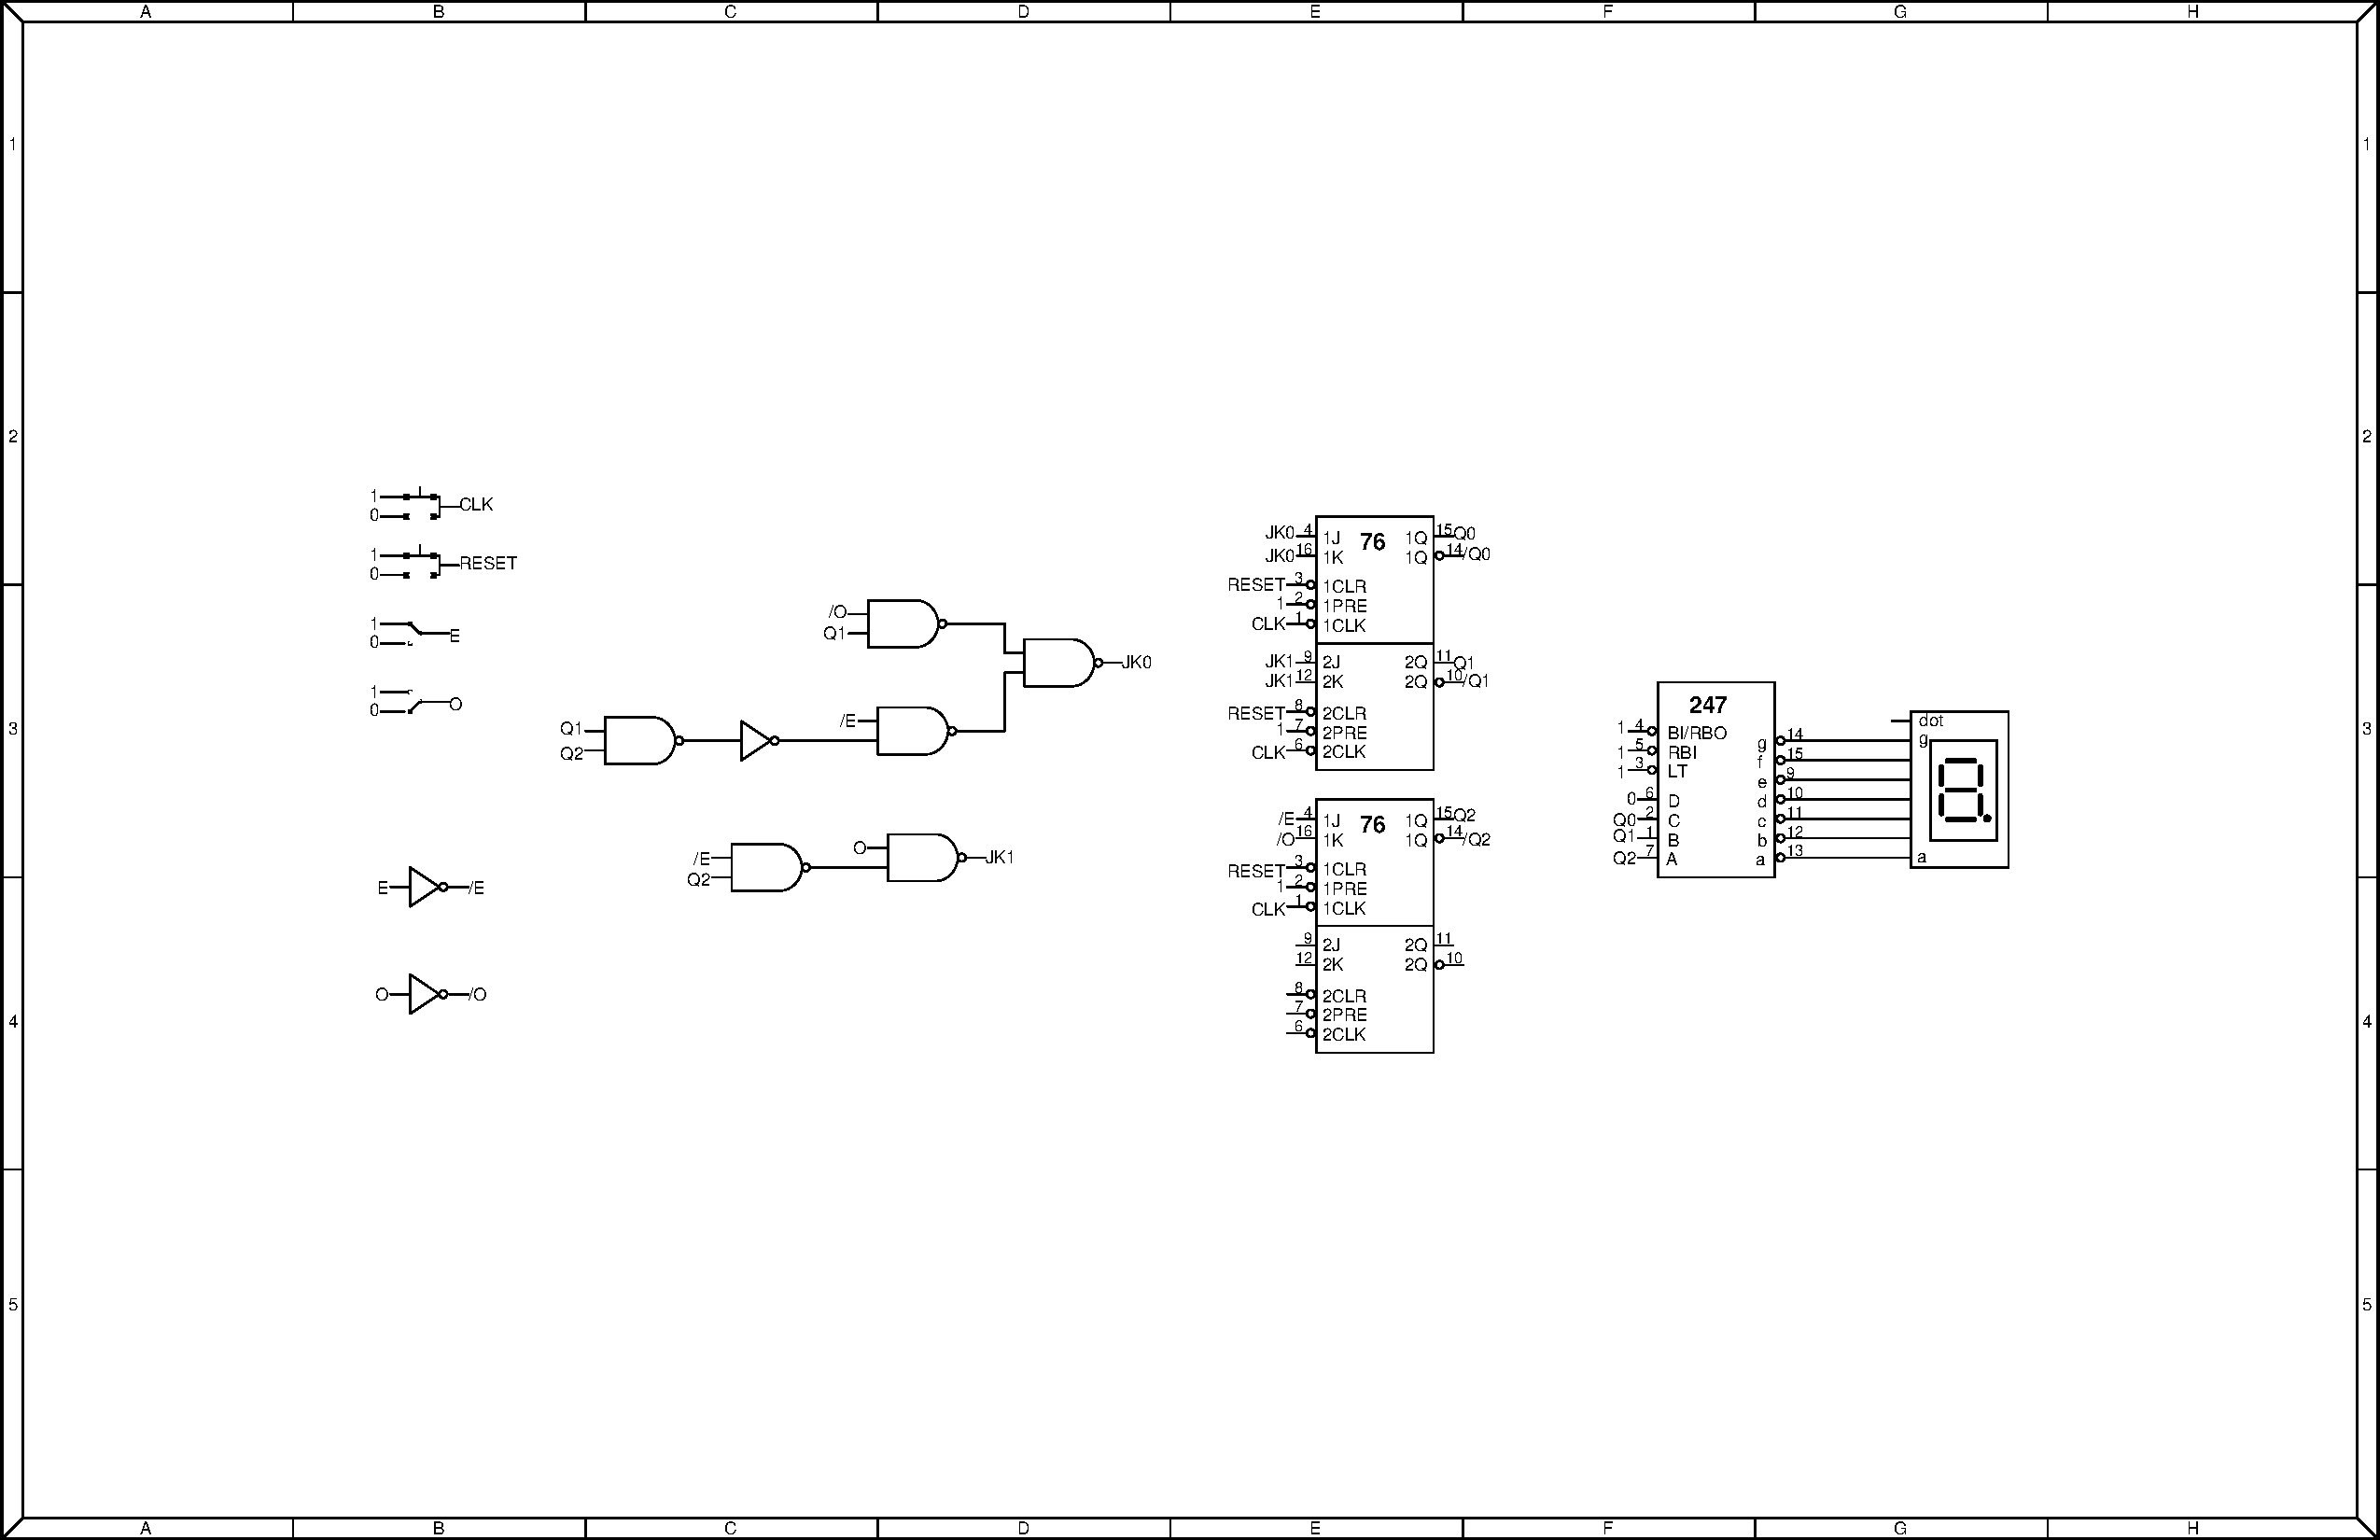
\includepdf[landscape=true, pages=-, scale=0.97]{jksimulation.pdf}
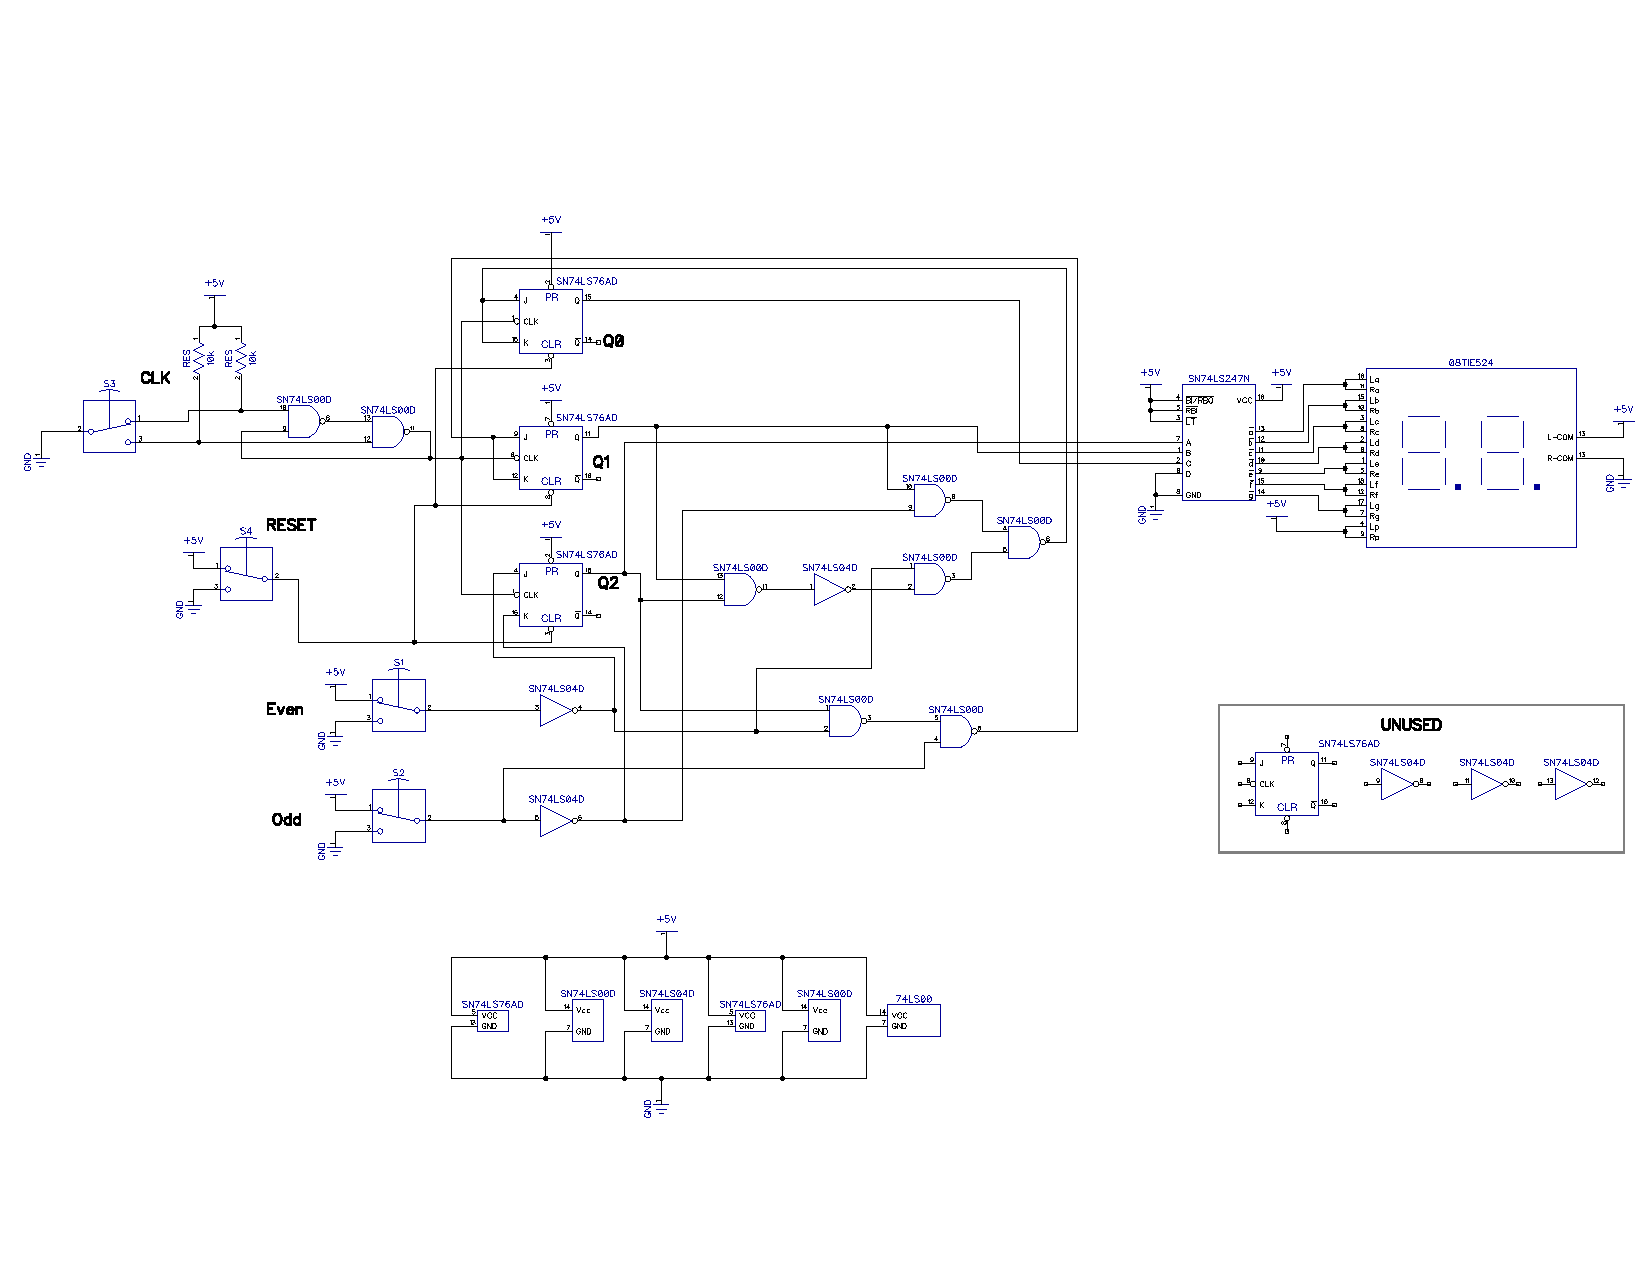
\includepdf[landscape=true, pages=-, scale=0.97]{jkschematic.pdf}

\section*{Results}

This laboratory took us longer to complete than it should have. Our first design involved using D flip-flops. The minimized logic into into the D flip-flops called for 27 NAND Gates and 8 NOT Gates. We got about halfway through wiring this when we decided to do out the karnaugh maps for the JK flip-flop logic also which turned out to be much, much smaller. Also, we realized that we needed a clear button for the flip-flops. We discovered this when trying simulate the circuit that the simulation would not work unless we first sent a clear signal to the flip-flops. Most other minor problems, such as incorrectly converting to NAND gates, were discovered while simulating the circuit. The final circuit worked perfectly and the SR Latch produced a perfect debounce for the toggle.

\section*{Conclusions}

A three bit counter can very easily be constructed with three JK flipflops and a small amount of sequential logic. The karnaugh maps for the JK flipflops seemed intimidating but turned out to minimise a lot better than the D flipflop karnaugh maps.

\section*{FTQ}

\textit{Question: If you�re counting 0 to 15, how many possible states are there for each combination of even/odd input signals? How many flipflops would you need?}
\\ \\
    There are four possible combinations of input signals: None, Even, Odd, Both. Since there are 16 states (0 to 15) for each combination of input signals, there are 64 possible states in total. Four flipflops would be needed to represent 15.

\end{document}
